\documentclass[12pt,oneside,final]{siuethesis}
\usepackage{microtype} % (optional) for more beautiful typesetting
\usepackage{graphicx} 
\usepackage{hyperref} %makes links clickable
\hypersetup{colorlinks,citecolor=black,filecolor=black,linkcolor=blue,urlcolor=black} %good for electronic copy
\hypersetup{colorlinks,citecolor=black,filecolor=black,linkcolor=black,urlcolor=black}%required for paper graduate school copy
%\usepackage[alphabetic]{amsrefs} %required if using amsrefs, comment out if using bibtex
\usepackage{fixltx2e}
\usepackage{amsmath}
\usepackage{epsf}
%\usepackage{float}
\usepackage{caption}
\usepackage{subfig}
%\usepackage{subcaption}
\usepackage{listings}
\usepackage{rotating}
\usepackage{tabularx}

\usepackage{multirow}

%% controls numbering of theorems
%% this can be configured to your advisor's taste
\newtheorem{theorem}{Theorem}[chapter] %theorem number resets each chapter
\newtheorem{conclusion}[theorem]{Conclusion}
\newtheorem{condition}[theorem]{Condition}
%% conjectures, corollary, defn, etc. numbered sequentially from beginning of chapters
\newtheorem{conjecture}[theorem]{Conjecture} 
\newtheorem{corollary}[theorem]{Corollary}
\newtheorem{example}[theorem]{Example} 
\newtheorem{lemma}[theorem]{Lemma}
\newtheorem{proposition}[theorem]{Proposition}
\newtheorem{solution}[theorem]{Solution}
\theoremstyle{definition}
\newtheorem{definition}[theorem]{Definition}


\author{Bryan Orabutt}
\title{Design of a Multichannel Constant Fraction Discriminator IC for Use in Nuclear Physics Applications}

%%\advisor{John Q.\ Faculty} %% or 
\advisor{Dr.}{George L. Engel}
\secondreader{Dr.}{Bradley Noble} %% or \secondreader{Dr.}{Karl Gauss}
\thirdreader{Dr.}{Timothy York}
%\fourthreader{Karl Gauss, Sr.}
%\fifthreader{Karl Gauss, Sr.}
%\secondadvisor{Karl Gauss} %if you haves two advisors (rare) then use this line also and pass the option `twoadvisors' to the class
%\abstracttext{Chairperson: The Honorable Jill Smith} %optional -- you can use this to override the text on the abstract page; the grad school default is built-in
\submitdate{April, 2018} %date the month/year submitted to grad school, use a comma between
\copyrightyear{2018} %optional, but required if copyrighted

%% all of these are optional; defaults are shown
\major{Electrical Engineering} 
\degree{Master of Science} %can be used to specify M.A., etc.
\highestdegree{Bachelor of Science} %used if the author already has another graduate degree
\department{Electrical and Computer Engineering} 
%\departmentname{Department}
%\refname{REFERENCES} 

%\captionsetup{width=0.7\textwidth}

\begin{document}
\maketitle 

\frontmatter %signals single spacing/roman numeral pagination

\copyrightpage %optional

%%% abstracts are optional
\begin{abstract}
\par This thesis presents the design and simulation of a multichannel integrated circuit (IC) that will be used in nuclear physics experiments. The chip is being designed as a companion chip for another IC used in particle identification called PSD8C. The IC described in this thesis is used create precise timing pulses for starting time-to-voltage converters (TVCs) on the PSD8C. These timing pulses are created using a technique called constant fraction discrimination. Each of the sixteen channels in the IC contains a Nowlin circuit, leading edge discriminator, zero cross discriminator, and a one shot circuit to generate the output. \par The IC will support input pulse amplitudes between 20 mV and 2V both positive and negative, and input rise times between 3 nsec and 100 nsec. The IC will feature a programmable output pulse width between 50 nsec and 500 nsec. Most importantly the output pulse firing time variation will be independent of the input amplitude and rise time, having a time walk of only 1 nsec or less. The IC has been named CFD16C and the design presented is using the AMI 0.5 micron NWELL process.

\end{abstract}

\begin{acknowledgements}

\par I would first like to thank Dr. George Engel for being a continuous source of guidance through all my time working on this project. I would also like to thank Dr. Bradley Noble for encouraging me to investigate challenging problems and for being a source of guidance both in the classroom and out. I would also thank Dr. Timothy York for introducing me to IC design, without him I likely would never have gone to graduate school. Additionally, Dr. Gary Mayer of the Computer Science department has helped me expand knowledge beyond the skills learned in the classroom, and I am forever thankful.
\par I would like to thank the other graduate students I've been privileged to work with on this project as well. Pohan Wang, Prarthana Jani, Sneha Edula, and Anil Korkmaz. We all worked together to make CFD16C possible and they have helped make this project a pleasure to work on.
\par I would like to thank my friends Jack White, Jared Charter, and Cameron Costanzo, Nelly Sanchez, and Shana Mankouski for helping me get to this point, each in their own ways. Finally I am forever grateful to my family for being a constant source of encouragement. My mother Marsha Orabutt, brother Sean Orabutt, and the woman who has been like a second mother to me, Vicki Kern, have been there for me and I know I could not have come this far without them.

\end{acknowledgements}

\tableofcontents

\cleardoublepage %cause correct numbering of list of figures

\listoffigures %print list of figures page

\cleardoublepage

\listoftables

\mainmatter %signals single spacing/arabic numeral paginations


\chapter{INTRODUCTION}  %% chapter titles must be typed in all caps to conform with regulations
\section{Background}
\par This thesis presents the initial design of a multichannel integrated circuit (IC) for use in nuclear physics applications. The IC as of this writing has not been finished and development will continue in a newer design process. The IC will be capable of using constant fraction discrimination (CFD) to create output timing pulses that are independent of input voltage and rise time. The work on this IC has been made possible due to a grant from the National Science Foundation (NSF Grant\#1625499).
\par Collaboration with nuclear physics researchers at Washington University in St. Louis has allowed the design of CFD16C to meet the needs for any experiments involving the PSD8C. The CFD16C is being designed to have better jitter and time walk performance than current existing CFD circuits using VME interface as well as offer functionality tailored to nuclear physics experiments. Combined with its companion ICs the CFD16C will allow for more precise experiments that was previously available.

\section{Need for an Integrated Circuit}
\par There is a need for an IC containing multiple configurable CFD circuits. Other timing ICs and VME CFD circuits do not offer any custom tailored solutions to nuclear physics applications and can limit the scope of an experiment. An IC with the following features is desirable \cite{CFD}:

\begin{itemize}
\item 
Support for up to 16 detectors.
\item
Support amplitudes between 20 mV and 2 V  with between 3 nsec and 100 nsec rise times.
\item
Support for both positive and negative input pulse amplitudes.
\item
Output timing pulse should be independent of input amplitude and rise time.
\item
Configurable leading edge threshold value for each channel.
\item
Programmable output pulse width between 50 nsec and 500 nsec.
\item
Allow for 1 KHz pulse repetition rates.
\end{itemize}

\section{Previous Work}
\par The CFD16C integrated circuit described in this thesis is intended to be used with another microchip (called PSD8C) which employs a technique known as pulse shape discrimination \cite{HALL}. Below is a summarized description of the PSD8C \cite{PROCTOR}. The PSD8C contains eight channels, each containing a time-to-voltage converter (TVC) and three sub channels. The TVC circuits are configurable with two time ranges (0.5 $\mu$sec and 2 $\mu$sec). Each sub channel contains a gated integrator that can be configured with 8 different charging rates, as well as configurable gate generators to set the start and width of the gate relative to the CFD timing pulse (each with 4 time ranges). The PSD8C also has support for 3 triggering modes. The output of a PSD8C channel consists of four sparsified pulse trains (one TVC, three integrators) that are synchronized for digitization by an off chip analog to digital converter (ADC). A system level diagram of the PSD8C is shown in Figure~\ref{fig:PSD} \cite{PSD-NSF}.\newpage

\begin{figure}[ht]
\centering
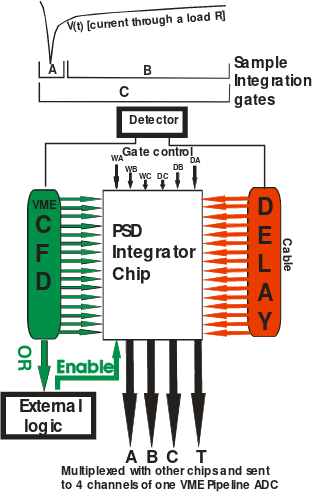
\includegraphics[scale=1,keepaspectratio=true]{images/PSD_block.png} 
\caption{System level overview for the PSD8C}
\label{fig:PSD}
\end{figure}

\par The PSD8C itself is a companion chip for another IC called HINP16C. It is useful to understand HINP16C as well in order to better understand the purpose of CFD16C. HINP16C contains 16 channels for use with silicon strip detectors \cite{HINP}. In each channel there is a charge sensitive amplifier (CSA) with two gain modes. In high gain mode the CSA has a gain of 15 $\frac{mV}{MeV}$ and in low gain it has a gain of 3 $\frac{mV}{MeV}$. The CSA outputs are split and act as inputs to energy and timing branches to produce sparsified pulse train outputs with synchronized addresses for an off chip ADC. 
\par The energy branch consists of a shaping filter that has a return to baseline time of under 20 $\mu$sec. This \emph{slow shaper} circuit is used as input to a continuous-time peak sampling circuit. The timing branch has a pseudo CFD circuit that uses a leading-edge and zero-crossing discriminator. The zero-crossing discriminator makes use of a DC offset cancellation loop to null out any unwanted DC offsets. A DAC is used to correct offsets in the leading-edge discriminator as well as set the CFD threshold level. This CFD output is used to start a TVC circuit with a configurable measurement range (250 nsec and 1 $\mu$sec). This TVC and the peak sampling circuit are reset after a user configurable delay time (referenced to the CFD firing time). A system level diagram of HINP16C is showed in Figure~\ref{fig:HINP} \cite{HINP-THESIS}.

\begin{figure}[ht]
\centering
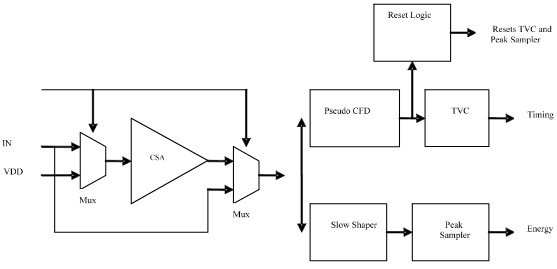
\includegraphics[scale=1,keepaspectratio=true]{images/HINP_block.png} 
\caption{System level overview for the HINP16C}
\label{fig:HINP}
\end{figure}

\section{Scope of Thesis}
The object of this thesis work was to begin the design and layout of essential analog elements of the CFD16C (Constant Fraction Discriminator - 16 Channels) integrated circuit. The CFD16C is a companion chip to accompany the PSD8C described in \cite{PROCTOR}. The CFD16C generates the timing pulses needed to start time-to-voltage converters on the PSD8C using a technique called constant fraction discrimination. Information about this technique can be found in \cite{NOWLIN}.
\par This thesis contains five chapters. Chapter 2 describes the system level overview of the CFD16C. Chapter 3 contains descriptions of the electronic circuits designed for the CFD16C. Chapter 4 contains simulation results showing the circuit elements described in chapter 3 function appropriately. Chapter 5 has a summary, conclusion, and description of future work to be done on the CFD16C.

\chapter{SYSTEM LEVEL DESIGN}
\section{Overview of Chip}
\par The CFD16C is designed in a 0.5 micron CMOS process. The chip is designed to act as a multichannel constant fraction discriminator with very low jitter and time walk in the output timing pulse. A system level block diagram of a single CFD channel can be seen in Figure~\ref{fig:CFD}.

\begin{figure}[ht]
\centering
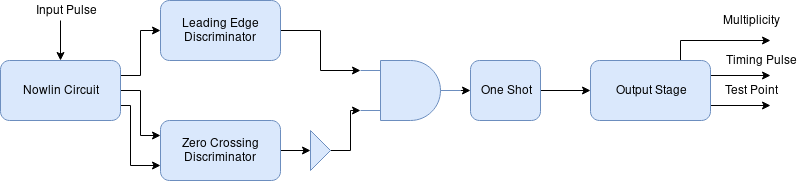
\includegraphics[scale=.55,keepaspectratio=true]{images/CFD.png} 
\caption{System level overview for one channel of the CFD16C}
\label{fig:CFD}
\end{figure}

\par An analog input pulse will arrive at the input stage of of the channel in the form of an exponential voltage pulse with a rise time ~10 times faster than its fall time. This input pulse goes to a Nowling circuit that creates a differential output and a high pass filtered output. The differential output is used as input to a zero crossing discriminator while the high pass filtered output is used as input to a leading edge discriminator. The outputs of the two discriminator channels are ANDed together to provide input to a one shot that creates the output timing pulse. Additional outputs such as a test point and multiplicity output are generated in a final output stage of the channel. 

\section{Features of CFD16C}
\par The CFD16C is being designed with several key features in mind to make it useful in experiments paired with the PSD8C. Below is a brief overview of the features that the CFD16C is intended to have when it is complete.

\begin{itemize}
\item
16 channels to support two PSD8C microchips for every one CFD16C.
\item
Supports positive and negative input voltages.
\item
Employs constant fraction discrimination to generate a low jitter output timing pulse.
\item
Time walk of output timing pulse must not exceed 1 nsec.
\item
Each channel has a configurable leading edge threshold.
\item
Delay time on Nowlin circuit globally configurable between 0.5 pF and 8 pF.
\item
Width of output timing pulse globally configurable between 50 nsec and 500 nsec.
\item
Provide test point outputs of key points in channel circuitry.
\item
Provide multiplicity output proportional to number of channels fired.
\item
Provide logical OR of all channel outputs.
\end{itemize}
\section{Common Channel}
\par The common channel of the CFD16C contains biasing circuits, two 5-bit configuration registers, multiplicty output, and channel OR output. One of the configuration registers is used to set the value of a programmable capacitor of the Nowlin circuit in every channel as well as provide negative polarity control for the leading edge threshold DAC. The second register is used to select the channel that the test point pad is connected and another bit to enable or disable a lockout time on the oneshot circuit.  Tables~\ref{Tab:reg1}-\ref{Tab:reg2} describe the register settings.
\begin{table}[h]
\parbox{.45\linewidth}{
\centering
	\begin{tabular}{|l|p{4cm}|}
		\hline
		Bit Position & Purpose\\\hline
		0-3 &Programmable capacitor\\\hline
		4 & Negative polarity.\\\hline
	\end{tabular}
    \caption{Register 0 functionality.}
 	\label{Tab:reg1}
 	}
 	\hfill
\parbox{.45\linewidth}{
	\begin{tabular}{|l|p{4cm}|}
		\hline
		Bit Position & Purpose\\\hline
		0-3 & Test point channel.\\\hline
		4 & Lockout enable..\\\hline
	\end{tabular}
    \caption{Register 1 functionality.}
 	\label{Tab:reg2}
    }
\end{table}

\section{CFD Channel}
\par The CFD16C contains 16 CFD channels used to generate a narrow timing pulse. This timing pulse is used to accurately mark the arrival of an analog input pulse for the PSD8C microchip. The channel design illustrated in Figure~\ref{fig:CFD} contains a Nowlin circuit, zero crossing discriminator, a leading edge discriminator, and a one shot circuit to create the timing pulse.
\subsection{Nowlin Stage}
\par The Nowlin circuit is used to create a differential output. One leg of this output is composed of a constant fraction of the input pulse. The other leg of this output is a delayed version of the input pulse. This delay time is determined by an RC time constant that is configurable by changing the value of a programmable capacitor. A high pass filter output is provided by the Nowlin as well, with a corner frequency of ~100 kHz. The Nowlin circuit is described in more detail in Chapter 3.
\subsection{Zero Crossing Discriminator Stage}
\par The differential outputs of the Nowlin circuit are used as inputs to a zero crossing discriminator. This discriminator is created by cascading three differential amplifiers together and connecting the final output to a high speed comparator. This circuit will provide a digital output that is a logic high (5V) when the two differential output voltages cross the 0V threshold when referenced to analog ground (AGND). This will allow the circuit to produce an output independent of the input pulse amplitude \cite{CFD}. 
\par To achieve amplitude independence it is important that the delay time set in the Nowlin circuit is optimal. With a short delay time there is very little under drive in the output of the final differential amplifier which could prevent the comparator from firing. With too much delay there is not enough slew rate to accommodate the fast timings that are needed (1 ns or less time walk and jitter). The importance of high slew rate is the reason fro cascading multiple differential amplifiers as opposed to using one high gain diff-amp. The amplifiers designed have a gain of ~5. For first order approximations it is known that the bandwidth of a differential amplifier obeys Eqn~\ref{eq:bw} \cite{CFD}.
\begin{eqnarray}
BW = \frac{0.35}{t_{10-90}}
\label{eq:bw}
\end{eqnarray}
\par The zero crossing discriminator needs an overall bandwidth of 50 Mhz. Since there are three diff-amp stages, each diff-amp needs a total bandwidth of $\sqrt{3} \approx 1.7$  times larger. This means the differential amplifiers needs a bandwidth of at least 85 Mhz in order for the zero cross discriminator to function properly. The final output of the comparator is delayed by 10 nsec in order to ensure the leading edge discriminator output fires first.
\begin{figure}[ht]
\centering
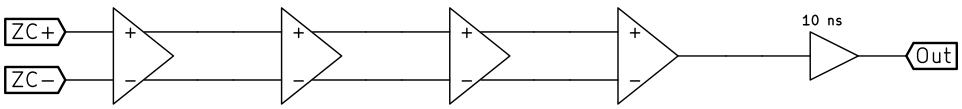
\includegraphics[scale=.55,keepaspectratio=true]{images/zcd.png} 
\caption{Zero crossing discriminator stage.}
\label{fig:ZCD}
\end{figure}
\subsection{Leading Edge Discriminator Stage}
\par The high pass filter output of the Nowlin is used as a input to a leading edge discriminator. This discriminator is comprised of a differential amplifier that connects to a differential to single ended amplifier with a gain of ~1. The differential amplifier helps remove common mode noise \cite{COMMON_MODE}. Removing noise is essential to improving the jitter as it is directly related to the input noise  as shown by Eqn~\ref{eq:jitter} \cite{CFD}. 
\begin{eqnarray}
\sigma _t  = \frac{\sigma _v}{SR}
\label{eq:jitter}
\end{eqnarray}
\par The output of the differential to single ended amplifier is compared against a user set threshold voltage that is generated by a 6-bit DAC. The DAC is used to set the noise floor threshold to give even greater noise immunity, as well as help nullify effects from offset voltages in the amplifier stages. Since the CFD channel can operate regardless of input voltage polarity, this DAC has a negative polarity control signal that when enabled (ie. 5V) will provide an output voltage that is below AGND. The same diff-amp and comparator circuits from the zero crossing discriminator circuit are used in the leading edge discriminator as well. 
\begin{figure}[ht]
\centering
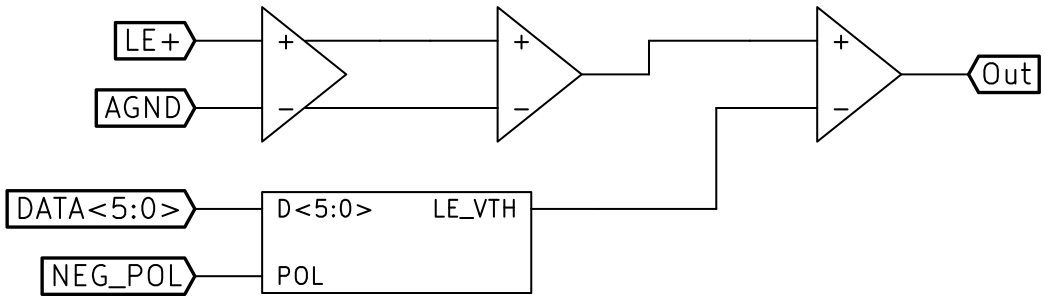
\includegraphics[scale=.55,keepaspectratio=true]{images/led.png} 
\caption{Leading edge discriminator stage.}
\label{fig:ZCD}
\end{figure}
\subsection{Oneshot Stage}
\par The timing pulse of each CFD channel is produced in the oneshot stage (Fig~\ref{fig:oneshot-stage}). This stage contains and edge detector, two oneshot circuits, and a 4-bit unipolar DAC. The input to the oneshot stage comes from the digital output pulses from the comparators in both the leading edge discriminator and zero crossing discriminator. 
\par The outputs of the two dicriminator stages are first ANDed together. Since the zero crossing discriminator (ZCD) stage is delayed, the leading edge discriminator stage (LED) can be used as a qualifier. The AND of these two thus guarantees that the output of the ZCD is from a real input pulse and not random transients. The ANDed discriminator signals are then used as input to an edge detector whose output triggers a oneshot circuit.
\par A oneshot circuit is a circuit whose input is a narrow pulse and outputs a fixed width pulse \cite{ONESHOT}. There are two oneshots in this stage. The first one creates the timing pulse that will eventually be output to the CFD16C output pad for the channel. The second oneshot is triggered by the first, and creates a lockout timing pulse to prevent the first oneshot from firing for a fixed amount of time. The width of the timing pulse is determined by a 4-bit logarithmically distributed digital-to-analog converter (DAC) with timing values shown in Table~\ref{Tab:oneshot-pw}. The lockout oneshot has its pulse width determined by an analog control voltage that is generated off chip.
\vspace{0.25in}
\begin{table}[h]
\centering
	\begin{tabular}{|l|p{4cm}|}
		\hline
		Digital Value (V) & Pulse Width (nsec)\\\hline
		0 & 500\\\hline
		1 & 250\\\hline
		2 & 100\\\hline
		3 & 50\\\hline
	\end{tabular}
    \caption{DAC digital code word to oneshot pulse width mapping.}
 	\label{Tab:oneshot-pw}
\end{table}
\newpage
\begin{figure}[ht]
\centering
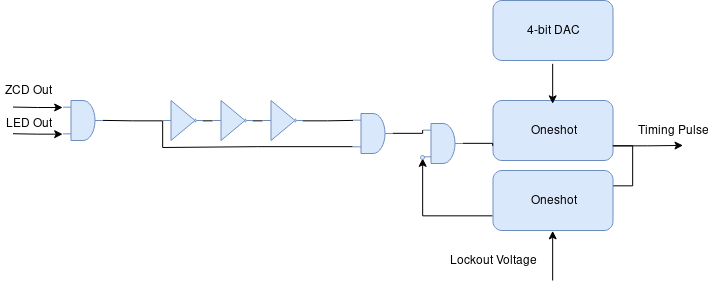
\includegraphics[scale=.55,keepaspectratio=true]{images/oneshot_stage.png} 
\caption{Oneshot stage.}
\label{fig:oneshot-stage}
\end{figure}
\subsection{Output Stage}
\par The timing pulse output is generated by a one shot circuit that fires a fixed width output pulse in response to a narrow input pulse that is created by an edge detector. All of the channel outputs are generated in a final output stage that contains a configuration register and an analog mutliplexer. The channels provide two other outputs to the user:  a multiplicity output that provides an analog voltage proportional to the number of channels that have fired, and a test point output that can be configured to select several points of interest from within the channel to present on the output pad. The output stage also contains a qualifier circuit that compares the output of the channel with a global enable pin, and a channel enable register bit.
\vspace{0.25in}
\begin{figure}[ht]
\centering
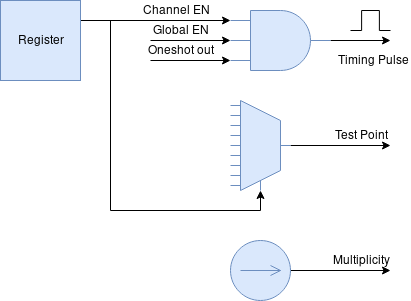
\includegraphics[scale=.6,keepaspectratio=true]{images/output_stage.png} 
\caption{Output generation stage overview.}
\label{fig:output-stage}
\end{figure}
%Table from image: 

%\begin{table}[htbp!]
% \centering
 %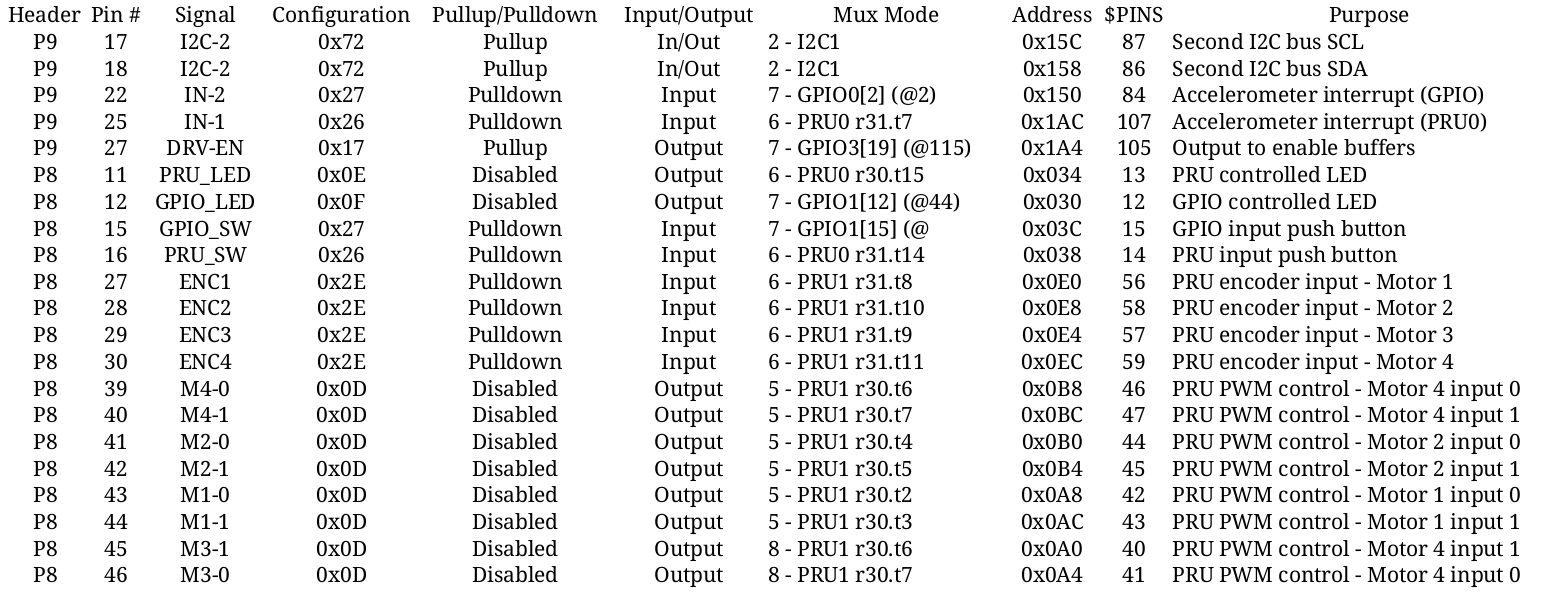
\includegraphics[scale=.3,keepaspectratio=true]{./images/Pinlist.png}
 %\caption{BeagleBone Black Pins Used by SIpeUE Robot Cape}
 %\label{tab:Pin_list}
%\end{table}

\chapter{CIRCUIT LEVEL DESIGN}

\section{Process Parameters}
%Equation Array:

%\begin{eqnarray}
%pwm(n) &=& pwm(n-1) + \Delta(n) \\
%\Delta(n) &=& \Delta_p(n) + \Delta_i(n) + \Delta_d(n) \nonumber \\
%\Delta_p(n) &=& K_p \cdot e(n) \nonumber \\
%\Delta_i(n) &=& K_i \cdot \left[ e(n) - e(n-1) \right] \nonumber \\
%\Delta_d(n) &=& K_d \cdot \left[ e(n) - e(n-1) + 2 \cdot e(n-2) \right] \nonumber
%\end{eqnarray}

\section{Common Channel}

\section{Digital Configuration}

\section{Bandgap Reference}

\section{Bias Currents}

\section{Nowlin Circuit}

\section{Differential Amplifier}

\section{Comparator}

\section{Oneshot Circuit}

\section{Output Generation}

\chapter{SIMULATION}
\section{Methods}
\par This chapter presents simulated data for many of the circuits designed for the CFD16C. This data was acquired using the Spectre simulator with Verilog-A test bench fixtures that produced stimuli for circuit level devices. The data presented represents ideal circumstances. More thorough simulation data will be obtained in the future when the IC is closer to completion.

\section{Configuration Registers}

\section{Bandgap}

\section{Oneshot}

\section{Nowlin}

\section{Differential Amplifier}

\section{Comparator}

\section{Zero Crossing Discriminator}

\section{Leading Edge Discriminator}

\section{Walk Analysis}

\chapter{SUMMARY, CONCLUSIONS, AND FUTURE WORK}

\section{Summary}



\section{Conclusions}



\section{Future Work}

\references %single spacing / arabic numeral paginations, adds "REFERENCES" to table of contents

%%%% for bibtex

%If you want to use bibtex  use the following lines, where your .bib file is called 'yourbib.bib'

\bibliographystyle{apalike}
\bibliography{./borabut_thesis.bib}

% If you have only a single appendix, do it this way.

\multipleappendices
\lstset{
         language=C,
         basicstyle=\scriptsize\ttfamily,
         emptylines=0, 
         lineskip=1pt,
         %numbers=left,            
         numberstyle=\tiny,         
         stepnumber=2,              
         numbersep=5pt,             
         tabsize=3,                
         extendedchars=true,       
         breaklines=true,            
         commentstyle=\color{blue},
         keywordstyle=\color{red},
            frame=b,         
 %        keywordstyle=[1]\textbf,    
 %        keywordstyle=[2]\textbf,    
 %        keywordstyle=[3]\textbf,  
 %        keywordstyle=[4]\textbf,   \
         stringstyle=\scriptsize\color{green}\ttfamily, 
         showspaces=false,         
         showtabs=false,            
%         xleftmargin=17pt,
%         framexleftmargin=17pt,
%         framexrightmargin=5pt,
%         framexbottommargin=4pt,
         %backgroundcolor=\color{lightgray},
         showstringspaces=false           
 }

\chapter{Verilog-A Code}

\end{document}